%\documentclass{imposter}
\documentclass[landscape]{imposter}
\bibliographystyle{plain}
\usepackage{layout}
\usepackage{amsmath}
\title{Compatible finite element methods for geophysical fluid dynamics}
\author{Colin J. Cotter}
\department{Department of Mathematics}
\institution{Imperial College London}
\email{colin.cotter@imperial.ac.uk}
\url{http://www.imperial.ac.uk/people/colin.cotter}
\def\MM#1{\boldsymbol{#1}}
\def\pgfsysdriver{pgfsys-dvipdfm.def}
\usepackage{amscd}
\usepackage{multicol}
\setlength{\columnsep}{1.5cm}
%% Primary university logo.
\logo{imperial.eps}
% Secondary logos (not supported in all poster styles)
\logoa{}

%% Options to set colors of multiple poster features.
%\titlecolor{named}{Blue}
%\postercolor{named}{Red}
%\pagecolor{green}

%% Overall poster themes.
%\posterstyle{tudelftstyle} % Official TU House style.
%\posterstyle{tudelftlandscape} % This requires the 
                                % landscape documentclass option
\posterstyle{amcgstyle} % Amcg poster with amcg logo in blue block
% at bottom.
%\posterstyle{amcgstyle} % Amcg poster with amcg logo in blue block at bottom.

% Use group with amcgstyle to specify a different group name.
\group{The Gung Ho Project}
% Use group with amcgstyle to specify a project name other than Imperial
% College Ocean Model.
\project{{Firedrake http://firedrakeproject.org}}

% This defines the command \showgrid. Use this to get a background grid to
% your poster text area. This helps when positioning poster contents with
% \rput.
\newpsobject{showgrid}{psgrid}{subgriddiv=1,griddots=10,gridlabels=20pt}

% This sets up boxes to have nice rounded corners and somewhat thicker lines
% than the default.
\psset{linecolor=amcgdarkblue,linewidth=.2,cornersize=absolute,linearc=1.0,framesep=0.5}


\begin{document}
\begin{multicols*}{3}
\section{Introduction}
Compatible finite elements form the basis of the Gung Ho dynamical
core formulation, since they extend C-grid staggering to consistent
schemes on pseudo-uniform meshes that avoid the parallel computation
bottleneck caused by the poles in a latitude-longitude grid. They are
also very suitable for multiresolution meshes for seamless
basin-to-coast ocean modelling.

\section{What are compatible finite elements useful for?}

Compatible finite elements \cite{cotter2012mixed} reproduce the
following essential properties of the C-grid staggering when applied
to the linear shallow water equations on the $f$-plane:
\begin{multicols}{2}
\begin{enumerate}
\item No spurious pressure modes,
\item No spurious inertial oscillations,
\item Steady geostrophic modes,
\item Conservation of linear energy.
\end{enumerate}
\end{multicols}
In addition, compatible finite elements have the following advantages:
\begin{enumerate}
\item No orthogonality requirements on meshes; can use triangles or
  quadrilaterals (or combination).
\item Consistent discretisation of Coriolis, and higher-order options.
\item Flexibility to avoid spurious C-grid type inertia-gravity modes on triangles \cite{danilov2010utility}
  by selecting velocity/pressure degree of freedom ratio.
\end{enumerate}
This makes compatible finite element methods an attractive option for
seamless ocean modelling on multiresolution unstructured meshes.

\section{What are compatible finite element methods?}

Sets/spaces of finite element functions are defined by:
\begin{enumerate}
\item The choice of polynomials used in each cell (e.g., linear,
  quadratic, etc.),
\item The continuity constraints on the functions between neighbouring
  cells.
\end{enumerate}
In the compatible finite element framework, we choose:
\begin{enumerate}
  \item Continuity in normal component for velocity space $V_1$.
  \item Discontinuous functions for pressure space $V_2$.
\end{enumerate}
In addition we require that $\MM{u}\in V_1 \implies
\nabla\cdot\MM{u}\in V_2$, plus the existence of bounded operators
$\pi_1$, $\pi_2$ such that the following diagram commutes:
\begin{equation}
  \begin{CD}
H({\rm div})     @>\nabla\cdot >>  L^2 \\
@VV\pi_1V        @VV\pi_2 V\\
V_1     @>\nabla\cdot>>  V_2
\end{CD}
\end{equation}
The following examples all avoid spurious inertia-gravity modes.\vspace{1cm}
\\
\parbox{25cm}{\hrule height 0pt width 0pt
  {\bfseries RT0-DG0 on quads.}
RT0: In reference element, $x$-component is linear in $x$, constant in
$y$; $y$ component is linear in $y$, constant in
$x$. DG0: constant functions.}
\hspace{1cm}
\parbox{5cm}
       {\hrule height 0pt width 0pt 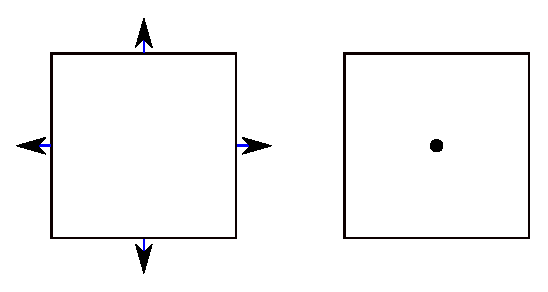
\includegraphics{RT0Q0DOFS}}
       \vspace{1cm} \\
\parbox{25cm}{\hrule height 0pt width 0pt {\bfseries RT1-DG1 on quads.}
RT1: In reference element, $x$-component is quadratic in $x$, linear in
$y$; $y$ component is quadratic in $y$, linear in
$x$. DG1: bilinear functions. Extension to higher order: RTk-DGk.}
\hspace{1cm}
\parbox{25cm}{\hrule height 0pt width 0pt 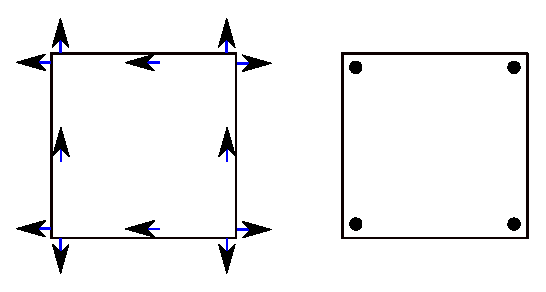
\includegraphics{RT1Q1DOFS}}
\vspace{1cm} \\
\parbox{25cm}{\hrule height 0pt width 0pt {\bfseries BDM1-DG0 on triangles.}
  BDM1: Linear vector-valued functions. DG0: constant functions.}
\hspace{1cm}
\parbox{25cm}{\hrule height 0pt width 0pt 
\includegraphics{BDM1_DOFS}} \vspace{1cm} \\
\parbox{25cm}{\hrule height 0pt width 0pt {\bfseries BDM2-DG1 on triangles.}
BDM2: Quadratic vector-valued functions. DG1: Linear functions. Extension
to higher-order: BDMk-DG(k-1).}
\hspace{1cm}
\parbox{25cm}{\hrule height 0pt width 0pt \includegraphics{BDM2_DOFS}}
\vspace{1cm} \\
\parbox{25cm}{\hrule height 0pt width 0pt {\bfseries BDFM1-DG1 on triangles.}  BDFM1: Quadratic vector-valued functions
    with normal components constrained to be linear on edges. DG1:
    Linear functions.}
\hspace{1cm}
\parbox{25cm}{\hrule height 0pt width 0pt
\includegraphics{BDFM1_DOFS}}\\
%Steady geostrophic modes

%Energy enstrophy conservation

%Vertical discretisation

%limiters
\small
\bibliography{seamlessocean}
\end{multicols*}
\end{document}
